
\documentclass[titlepage,12pt,a4paper]{article}

\usepackage[tc]{titlepic}
\usepackage{graphicx}

 \titlepic{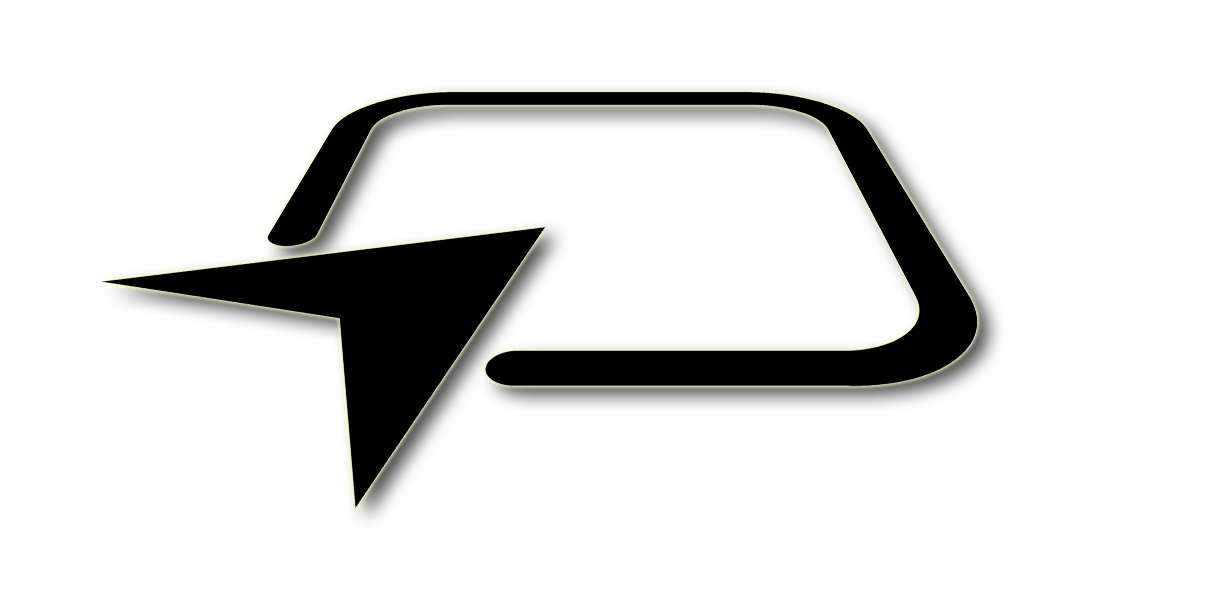
\includegraphics[width=\textwidth]{cover.png}}
 \title{\Huge \textbf{Kinetic Space}\\\Large~\\User Manual}
 \author{}
 \date{}

 \setlength{\parindent}{0pt}
 \setlength{\parskip}{5pt plus 2pt minus 1pt}
 \frenchspacing
 \sloppy

\begin{document}
 \maketitle
 \begin{abstract}

The \emph{Kinetic Space} provides a tool which allows everybody to record 
and recognize customized gestures using depth images as provided by  
PrimeSense's PS1080, the Kinect or the Xtion sensors. Five
highlights of the software are that the gestures

\begin{itemize}
	\item \emph{can be easily trained}\\ the user can simply train the system 
      by recording the movement 

	\item \emph{are person independent}\\ the system can be trained by one 
      person and used by others 

	\item \emph{are orientation independent}\\ the system can recognize gestures even if the trained and tested gesture does not have the same orientations 

	\item \emph{are speed independent}\\ the system is able to recognize the
      gesture also if it is performed faster or slower compared to the training 

	\item \emph{can be adjusted}\\ the system and gesture configuration can be setup by a XML file
\end{itemize}

The software has already been used by media artists, dancers and alike to 
control third party software such as Max/MSP, Pure Data, VVVV, Resolume, etc. 
via the OSC protocol. The software is written in Processing and based on 
SimpleOpenNI, OpenNI and NITE.
 
 \end{abstract}
 \tableofcontents

\newpage

 \section{Introduction}

The \emph{Kinetic Space} provides a tool which allows everybody to record 
and recognize customized gestures using depth images as provided by  
PrimeSense's PS1080, the Kinect or the Xtion sensors. The software observes and comprehends the user interaction by processing the skeleton of the user\footnote{two users are supported, but more users can be simply added by small changes in the source code}. The unique analysis routines allow to not only detect simple gestures such as pushing, clicking, forming a circle or waving, but also to recognize more complicated gestures as, for instance, used in dance performances or sign language.

Five highlights of the software are that the gestures:

\begin{itemize}
	\item \emph{can be easily trained}\\ the user can simply train the system 
      by recording the movement/gesture to be detected without having to write a single line of code 

	\item \emph{are person independent}\\ the system can be trained by one 
      person and used by others 

	\item \emph{are orientation independent}\\ the system can recognize gestures even if the trained and tested gesture does not have the same orientations of the person towards the sensor

	\item \emph{are speed independent}\\ the system is able to recognize the
      gesture also if it is performed faster or slower compared to the training and is able to provide this information

	\item \emph{can be adjusted}\\ the system and gesture configuration can be setup by a XML file; e.g. for one gesture to be recognized it can be set orientation independent while for other gestures it is orientation dependent
\end{itemize}

The software has already been used by media artists, dancers and alike to 
connect and to control a wide range of third party applications/software such as Max/MSP, Pure Data, VVVV, Resolume, etc. 
via the OSC protocol. The software is written in Processing and based on 
SimpleOpenNI, OpenNI and NITE.

More information about the project and the source code can be found at (reading this manual you probably have already done so) \\
\texttt{http://kineticspace.googlecode.com}.

To get a quick overview about the project check out the short video introduction about the functionality of \emph{Kinetic Space} at \\ \texttt{http://www.youtube.com/watch?v=e0c2B3PBvRw}.

\subsection{What the Press is Saying}
\emph{[...] What is it good for? Well, it can read a gesture from one person and register it on another and you can train it to register tiny movements and, potentially, allow for full motion control of your PC. Minority Report it isn't, but that future is getting closer and closer.}\\
--- www.techcrunch.com 2011/08/05

\emph{Map your gestures and have it ready for other people to use and make reference of. The Kinect Spaces is a gesture recognition and mapping software that gives programmers a reliable tool in creating and saving gestures via Kinect for their software use. This video by Matthias Wölfel shows us the nitty-gritty details of the program as well as how the Kinect Space can prove to be valuable to all Kinect hackers out there. [...] This is indeed a great addition in further enhancing the Kinect controls!}\\
--- www.kinecthacks.com 2011/07/21

\subsection{About the Logo}

The \emph{Kinetic Space} logo represents a space (represented by the box) with an arrow directing into the space, meaning please enter the \emph{Kinetic Space}.

\subsection{How to Support this Project}
Like any other open source project the success is based on the support of the community. There are a variety of possibilities: use the software, tell a friend, give feedback (positive or negative), work on the source code or documentation (please coordinate your activity) or provide financial support.

\newpage

 \section{Installation}

The \emph{Kinetic Space} is intended as an open system so that everybody has access to the full source code and that everybody can make adjustments to their own needs. Therefore, it does not come in binary form. Instead the program has been written in \emph{processing}\footnote{an open source programming language and environment} which can run on several platforms such as Linux, Mac OS X, and Windows (it has been sucessfully tested and used on all three platforms). 

To make the software run on your system, you have to install OpenNI\footnote{\texttt{http://www.openni.org/downloadfiles}} and PrimeSense's Natural Interaction Middleware (NITE)\footnote{\texttt{http://www.primesense.com/?p=515}}. In addition you have to install Processing\footnote{\texttt{http://processing.org}} with the following packages installed in the \texttt{libraries} folder:
\begin{itemize}
	\item SimpleOpenNI\footnote{\texttt{http://code.google.com/p/simple-openni}} --- a simple OpenNI and NITE wrapper for processing
	\item oscP5\footnote{\texttt{http://www.sojamo.de/libraries/oscP5/index.html}} --- an implementation of the OSC protocol for processing
	\item fullscreen\footnote{\texttt{http://www.superduper.org/processing}} --- better full screen support for processing
\end{itemize}

A detailed step by step instruction on how to install most of the used software, except oscP5 and fullscreen, for Windows, OS X and Linux can be found at the following link:\\ \texttt{http://code.google.com/p/simple-openni/wiki/Installation}.

Now, finally, you are able to load the source code in processing and run the program.

\newpage

 \section{How To Use}

This section gives you a brief overview on how to use the software, how to train new gestures and how to set customized OSC messages.

 \subsection{Recognizing Gestures}

After running the source code you first have to be recognized by the system. There are two possibilities:
\begin{itemize}
	\item The first is to register yourself by holding up your hands (if autodetection is turned off). 
	\item The second is to 'just' move in front of the sensor (if autodetection is turned on).
\end{itemize}
Note that even though only a single person is shown on the registering screen a second person can always be registered by the system. If one or two persons are registered, the system is already ready to use and is constantly analysing the gestures. In case the user is getting out of range, an icon (in the users color) is prompted which points into the direction the user has to move to get back into the viewing range of the sensor.

By pushing the 
\begin{itemize}
	\item \texttt{d} key you can flip the images.
	\item \texttt{+} or \texttt{-} keys you can switch between a visualization of the cost matrix for the different learned gestures and the current observation (only for the first person).
\end{itemize}

\subsection{Training New Gestures}

The system can easily learn new gestures by pushing a key between \texttt{0} and \texttt{9}. If one of these keys has been pressed the last 25 frames (one second) of the first person are stored and the novel gesture is immediately ready to be used by both persons. If you want to recognize a gesture which is less than 25 frames long, you can adjust for the length using the XML setup (see Section~\ref{sec:xml}).

Please note that in the current setup, stored gestures are replaced by the newly trained gestures without warning.

\subsection{XML Setup}
\label{sec:xml}
This section describes the configuration of the XML setup file. The setup file has to be located in the \texttt{data} folder and named \texttt{setup.xml}.

\subsubsection{Basic Setup}
\label{sec:basic_setup}
In this section we discus how to setup the basic system and how to set values which determine the settings for all gestures:
\begin{itemize}
\item \emph{autodetection} \\autodetection allows you to switch \texttt{on} or \texttt{off} a preloaded bones model. In this case where a preloaded bones model is used it is not needed to register with the registration pose (might not work on Mac OS X). Note, while this can be very convenient, it might not lead to the best possible recognition results (in particular if the system is going to be used by a single person).
\begin{verbatim}
<autodetection>yes</autodetection>\end{verbatim}
\item \emph{multithreading} \\ multithreading can be turned \texttt{on} or \texttt{off} using the command \begin{verbatim}
<usemultithreading>yes</usemultithreading>\end{verbatim}
\item \emph{normalization} \\ two different normalization methods can be turned \texttt{on} or \texttt{off}\begin{verbatim}
<normalize>
    <size>yes</size>
    <rotation>yes</rotation>
</normalize>\end{verbatim}
The first method, \texttt{size}, normalizes the size of a person to a standard person (might always lead to the best possible recognition result if turned on). The second method, \texttt{rotation}, normalizes the rotation of the person to the sensor. Note that it is helpful to normalize the rotation to be independent of the orientation of the person to the sensor. If the gesture to be detected, however, has a rotational component, it is better to turn the normalization of the rotation off.

For example, a throwing gesture, should be independent of the orientation of the throwing direction (the orientation of the throw should be determined by other methods: e.g. triangulation between the current hand position and a former hand position), while in a dance performance the spin (and thus orientation to the sensor) might be of interest.
\item \emph{weight} \\ to adjust for the influence of the different axis and the overall sensitivity you can set different weighs to the different axis by\begin{verbatim}
<weight>
    <x>1.0</x>
    <y>0.5</y>
    <z>1.5</z>
</weight>\end{verbatim}
This is helpful, for instance, if you want to recognize a gesture where the precision of the z-axis has to be very precise, while the precision of the y-axis should be quite flexible. An example could be a throwing gesture, here the z-axis should have a high precision (in particular if rotation normalized), while the y-axis should be flexible (it should not matter if your hand is close or far away from your body).
\item \emph{body part} \\ to select the body part of focus you can use one out of three options, namely: \texttt{botharms}, \texttt{leftarm} or \texttt{rightarm} \begin{verbatim}
<bodypart>bothams</bodypart>
\end{verbatim}
Once again, thinking about a throwing gesture, the arm and hand position of the throwing arm should matter, while the position of the second hand and arm should not matter. In this case it would be helpful to give all weight to the throwing arm and no weight to the other arm. This can be established by, either, \texttt{leftarm}, if the throwing arm is on the left or \texttt{rightarm} if the throwing arm is on the right.
\end{itemize}
\subsubsection{Individual Gesture Setup}
While in the former, we have discussed how to adjust for the overall setup, in this section we describe how to adjust an individual pose. This is possible by using \texttt{gesture} and an \texttt{id} as you can see in the example:
\begin{verbatim}
<gesture>
    <id>2</id>
    <normalize_rotation>no</normalize_rotation>
    <bodypart>rightarm</bodypart>
    <weight>
        <x>0.5</x>
        <y>0.5</y>
        <z>1.5</z>
    </weight> 
</gesture> 
\end{verbatim}
If you compare to Section~\ref{sec:basic_setup} you see that the structure is identical, except for the \emph{normalization} where the complete construct is replaced by \texttt{normalize\_rotation}. 
This is due to the fact that the normalization of the size can only be turned on or off for all poses at the same time while it is possible to turn of the normalization of the rotation on and off for each individual pose.
Note that if a variable or an individual gesture is not determined, the basic values as defined in Section~\ref{sec:basic_setup} are used.

\subsection{Customize OSC Messages}

In order to customize your OSC messages to your own needs (the needs of your favored music or visualization tool) you can adjust the sample code as provided in the function: \texttt{void sendOSCEvent(int event, int person)}.

Note that you can already separate between the detected gestures/events and the person who performed the action. If you want to include other information such as speed of action or confidence you have to extend the code respectively.

In a future version it is planned to adjust for the OSC messages by a XML file similar to the one already discussed.

\newpage

 \section{Some Words about Gesture Recognition}

Gestures are expressive, meaningful body motions such as physical movements of the fingers, hands, arms, head, or body and also include facial expressions such as emotion, with the intention  
\begin{itemize}
	\item to communicate meaningful information (semiotic),
	\item to manipulate or to interact with the environment (ergotic), or
	\item to discover the environment through tactile experience (epistemic). 
\end{itemize}
The \emph{recognition of gestures} is the interpretation of human movement by computers via mathematical algorithms. Gesture recognition\footnote{While the term \emph{gesture recognition} includes the interpretation of a static posture, but is not limited to it, in the literature systems which can \emph{only} detect static posture are often falsely called gesture recognition systems instead of pose recognition systems. }, therefore, enables humans to interface with the machine and interact naturally with or without any mechanical devices. Using the concept of gesture recognition, it is for example possible to point a finger at the computer screen so that the cursor will move accordingly, to interpret sign language or to analyse dance moves.

The ability to track and recognize a person's movements can be achieved through various sensors. Some are vision based\footnote{we are not including touch sensitive surfaces based on cameras in our overview}, which will be discussed in more detail, or controller based. Controllers are, for example, the computer mouse, data gloves which detect hand position, movement and finger bending or the Wii remote control, which measures acceleration over time. Vision based recognition can rely on 
\begin{itemize}
	\item \emph{a single camera}\\ A “normal” camera can be used to recognize gestures. Although not necessarily as effective as the other types of cameras it allows for a wider accessibility.
	\item \emph{a stereo camera}\\ Two cameras positioned next to each other can be used to determine depth in the scene by corresponding points in the two images. 
	\item \emph{a camera array}\\ Similar to stereo cameras the relation between the cameras (which can be placed for example in each corner of a room) can be used to get a 3D representation of the environment.
	\item \emph{a time-of-flight cameras}\\ The depth is measured, more or less similar to radar or LIDAR, by measuring the travel time of a light pulse which can then be transferred into distance. 
	\item \emph{a structured-light 3D scanner}\\ A depth map (a variant of image-based 3D reconstruction) can be derived by using projected infrared light patterns and an analysis of what is being seen in an infrared camera (Peng et al. 2007). The Kinect-Sensor is a prominent example.
\end{itemize}
Note that each sensing technology differs in accuracy, resolution, latency, range of motion, user comfort, and cost and therefore has advantages and disadvantages which need to be considered for the very specific purpose of an application.

Gestures can be classified into different categories:
\begin{itemize}
	\item \emph{gesticulation}\\ spontaneous movements of hands and arms that accompany speech
	\item \emph{sign languages}\\ linguistic systems which are well defined.
	\item \emph{pantomimes}\\ gestures that depict objects or actions, with or without accompanying speech
	\item \emph{pointing}\\ directional indication through pointing has a very specific purpose in our society, to reference an object or location based on its position relative to ourselves. 
	\item \emph{emblems}\\ gestures (often culturally specific) such as “waving”, “thumbs up”, “V for victory”, and assorted rude gestures 
	\item \emph{dance}\\ following a specific pattern / expression
	\item \emph{sport}\\ particular movements according to a particular sportive activity such as Tennis or Golf
\end{itemize}

These different types of gestures can be readily used for a broad variety of human-computer-interaction:
\begin{itemize}
	\item gestures can serve as virtual controllers (remote control) to trigger events to control interactions within video games to try and make the game player's experience more interactive or immersive
	\item gestures can be analysed to identify wrong movements in dance, sports (e.g. katas), healthcare (e.g. lifting a box)  
	\item gestures can be used to identify the emotional state of the user
	\item similar to speech recognition, certain types of gesture can be transcribed into text by interpreting the sign language
\end{itemize}

\newpage

\section{Algorithms \& Co.}

In this section we briefly explain the basic algorithms to realize a gesture recognition system. A common gesture recognition system is composed of three components, namely, the sensor (as already discussed), the feature-extraction (also called front-end) and the analysis (also called back-end). While the front-end is responsible to extract the relevant features of the sensor signal the back-end is responsible for the detection of pose (for each frame\footnote{In our context a \emph{frame} is defined as a single image.}) and gesture (for an array of frames).

In the literature two different approaches to gesture recognition are common: model or appearance based. While model based methods use key elements of the body represented in 3D coordinates (x,y,z) such as joint angles in order to obtain several important parameters, appearance-based models use either image sequences, or certain features derived from these, as gesture templates. Model approach can again be separated into volumetric or skeletal models. While the former have been heavily used in off line algorithms the latter is commonly used for real time analysis of gestures due to the fact that only key parameters have to be analyzed. The techniques we describe here rely on key points which are represented in a 3D coordinate system (Cartesian coordinates). Based on the relative motion of these key points, gestures can be detected with high accuracy. The quality of the recognition system depends on a number of parameters including:
\begin{itemize}
	\item quality of the input (accuracy of the key points, camera position, ambient light)
	\item proper selection of features (e.g. if a hand gesture needs to be classified it is not particular useful to include the food position as a feature)
	\item frame rate (a higher frame rate allows for a better tracking)
	\item intra- and interpersonal variability\footnote{intrapersonal variability, in gesture recognition, is defined as the amount of variation in repeating a gesture by a single person, while interpersonal variability is the amount of variation in the performance of a gesture between different persons} of gestures (gestures are highly variable, from one person to another and from one example to another from the same person)
	\item quality of the detection algorithm
\end{itemize}

\subsection{Feature Extraction (Front-End)}

In pattern recognition feature extraction refers to the process of reducing the number of input parameters such that relevant information from the input data is preserved or extracted in order to perform a desired task while the other information has to be omitted. This reduction of parameters is required to prevent the use of large amount of memory and computation power, but more importantly to prevent the classification algorithm from over fitting to the training sample and therefore to generalizes poorly to new samples.

Because gestures are highly variable, from one person to another and from one example to another performed by the same person, it is essential to extract "the essence of the gesture," while information such as the height or size of a person or the t-shirt color is not relevant. Note as it is not possible to completely reduce the user specific information it is always a tradeoff between accuracy and generality -- the more accuracy desired, the more user specific training is required. 

\subsection{Optimal Features}
Best recognition results can be achieved when an expert constructs a set of application-dependent features. Those features can be constructed either 
\begin{itemize}
	\item based purely on expert knowledge, 
	\item data driven applying dimensionality reduction techniques such as principal components analysis, independent component analysis, or linear discriminant analysis, or
	\item a combination of both. 
\end{itemize}

For the purpose of gesture recognition time-varying sequence of parameters describing position, velocities, and angles of relevant body part are most useful. 
In an ideal world those features would be noise free, time invariant, person independent, orientation independent (depending on the application) and robust to conclusions. Of course this ideal world does not exist and one has to cope with this effects as best as possible. That means one tries to compensate for those effects using particular algorithms. To make the extracted information person independent it is helpful to scale the length of different key points to match an “average” person. To make the extracted features independent of the orientation of the person to the sensor it is helpful to compensate for the orientation by a well defiended rotation around the persons vertical-axis.

\subsection{Analysis}

Pose (static gestures), can be recognized without the consideration of temporal patterns and, therefore, a straightforward implementation using standard pattern recognition techniques such as cost functions, template matching, geometric feature classification, neural networks, or support vector machines can be used. In order to interpret movements (dynamic gesture) of the body, one has to classify “the message” the movements may express. Therefore, techniques are required which consider 
\begin{enumerate}
	\item the results from pose classification (on a frame-by-frame basis), and
	\item the temporal structure.
\end{enumerate}
The consideration of temporal structure is typically accomplished through time compressing templates, \emph{dynamic time warping} (DTW), \emph{hidden Markov models} (HMM)s, or Bayesian networks.

Note that hand-coded gestures only work for trivial systems such as waving. In general, gesture recognition system needs to be trained through learning. Learning, in this case, means that the free parameters are set/defined automatically by observation (training set).

\subsection{Pose Recognition using Cost Functions}
To detect a pose a comparison between the reference and the test sample has to be calculated. The type of calculation is defined by the objective function or cost function. Two widely used methods to calculate the difference between the reference signal and the test signal are 
\begin{itemize}
	\item the Euclidian distance and 
	\item the Mahalanobis distance.
\end{itemize}

While the \emph{Euclidean distance}
\[
	d(\mathbf{x},\mathbf{y}) = \sqrt{(\mathbf{x}-\mathbf{y})^T(\mathbf{x}-\mathbf{y})}
\]
is defined as the distance between two vectors $\mathbf{x}$ and $\mathbf{y}$ given by the Pythagorean formula the 
\emph{Mahalanobis distance} (Mahalanobis 1936)
\[
	d(\mathbf{x},\mathbf{y}) = \sqrt{(\mathbf{x}-\mathbf{\mu}_y)^T\mathbf{\Sigma}_y^{-1}(\mathbf{x}-\mathbf{\mu}_y)}
\]
calculates the distance between one vector $\mathbf{x}$ and a mean vector $\mathbf{\mu}_y$ and variance matrix $\mathbf{\Sigma}_y$  of the training data $\{\cdots\}_y$. Note that the samples of the training data have to be from the same gestures but performed a couple of times by one person or different persons.  

The skeleton, or part, of a person consists of a couple of reference points. The overall distance is therefore calculated by summing over all those points, represented as the vectors $\mathbf{x}$ (feature values of the observation) and $\mathbf{y}$ (feature values of the comparison).

\subsection{Gesture Recognition based on DTW}
DTW is a simple but powerful algorithm for measuring similarity between two sequences which may vary in speed and/or acceleration. This capability is very important to compare gesture patterns as the speed of a performed gesture is highly variable and can even be important for further analysis (e.g. in dance). 
The standard definition of DTW distance between two time series $\mathbf{x}_m$ and $\mathbf{y}_n$ (with $M$ and $N$ elements respectively and $n$ and $m$ representing the frame indexes) is
\[
	\phi(m,n) = \Phi(m,n) + \min{(\phi(m-1,n-1),\phi(m-1,n),\phi(m,n-1))}
\]
where $\phi(m,n)$  is a $(M+1) \times (N+1)$ matrix, $\phi(0,n)$  and $\phi(m,0)$ are initialized with infinity or zero, depending on the application, and $\phi(0,0)$ with zero. The cost function is denoted by $\Phi(m,n)$ and might be defined with the Eucleadean distance as defined in the previous section as $\Phi(m,n) = d(\mathbf{x}_m,\mathbf{y}_n)$. The overall cost of the DTW algorithm of the two series equals to $\phi(M+1,N+1)$. The cost matrix $\Phi(m,n)$ and the shortest path, determined by backtracking (see Section~\ref{sec:backtracking} for details), can be visualized in the \emph{Kinetic Space}. Those informations can be useful in analysing and comparing the current input and learned gesture.

\subsubsection{Constraints} 
Although the DTW is a very powerful algorithm, as it has been introduced in the previous section, it has to be adapted to not produce pathological results and optimized its performance for a particular task. The reason for those pathological results is an “unnatural” warping of the two time axes resulting in unintuitive alignments. In the worst case one single point in one time series could map onto a large subsection of another time series (this can for instance happen if a pose is compared to a gesture). 

To deal with these unwanted effects is to adjust the basic algorithm to the specific needs by the introduction of additional constraints. A couple of constraints are discussed next:
\begin{itemize}
	\item \emph{windowing}\\ A local constraint that prevents the “search path” to deviate too far from the diagonal path by enforcing the constraint \[m-nN/M<R\] where $R$ defines the size of the search path. 
	\item \emph{slope weighting}\\ Introduces a penalty term $\alpha>1$ to penalize off-diagonal path choices to prevent the path from being to steep or to shallow.
\[
	\phi(m,n) = \Phi(m,n) + \min{(\phi(m-1,n-1),\alpha\phi(m-1,n),\alpha\phi(m,n-1))}
\]
Larger values of $\alpha$ lead to paths that are closer to the diagonal than smaller values.
	\item \emph{step pattern}\\ Alternative step patterns to force horizontal, vertical or diagonal steps.
\end{itemize}

\subsubsection{Backtracking}
\label{sec:backtracking}
So far we have discussed a way to determine the smallest cost between the two input sequences. While this information is needed to determine which gesture in the training set is closest to the current gesture it does not tell you much about the speed between training and testing. This information has, already been determined, by DTW (for $\phi(m,0) = 0~\forall~m$). Once the accumulated cost matrix has been build the optimal 'walking path' can be determined by backtracking the stored nodes from the end point = (M; N) to the start point = (1; 1).

\newpage

\section{Copyright Notice}
Copyright (c) 2011-2012, Kinetic Space \& Matthias W\"olfel, \\
All rights reserved.

~\\

Redistribution and use in source and binary forms, with or without 
modification, are permitted provided that the following conditions are met:

\begin{itemize}
	\item Redistributions of source code must retain the above copyright notice, 
      this list of conditions and the following disclaimer.
	\item Redistributions in binary form must reproduce the above copyright notice, 
      this list of conditions and the following disclaimer in the documentation 
      and/or other materials provided with the distribution.
	\item Neither the name of the software nor the names of its contributors
      may be used to endorse or promote products derived from this software 
      without specific prior written permission.
	\item If the software is used in other software products, installations or for
	  research, it must always be cited as "Kinetic Space" and a reference 
	  to the souce code \texttt{http://kineticspace.googlecode.com} has to be given.
	  This form of citation does not require any permission.
	\item Adding a "Powered by Kinetic Space" logo \& text whenever an online video is posted. And send us a note about the post.
	\item Do not release commercial project with \emph{Kinetic Space}: \emph{Kinetic Space} is for non-commercial use only. Contact us if you want to build a commercial product using \emph{Kinetic Space} technologies.
\end{itemize}

THIS SOFTWARE IS PROVIDED BY THE COPYRIGHT HOLDERS AND CONTRIBUTORS "AS IS"
AND ANY EXPRESS OR IMPLIED WARRANTIES, INCLUDING, BUT NOT LIMITED TO, THE 
IMPLIED WARRANTIES OF MERCHANTABILITY AND FITNESS FOR A PARTICULAR PURPOSE
ARE DISCLAIMED. IN NO EVENT SHALL THE COPYRIGHT HOLDER OR CONTRIBUTORS BE
LIABLE FOR ANY DIRECT, INDIRECT, INCIDENTAL, SPECIAL, EXEMPLARY, OR
CONSEQUENTIAL DAMAGES (INCLUDING, BUT NOT LIMITED TO, PROCUREMENT OF
SUBSTITUTE GOODS OR SERVICES; LOSS OF USE, DATA, OR PROFITS; OR BUSINESS
INTERRUPTION) HOWEVER CAUSED AND ON ANY THEORY OF LIABILITY, WHETHER IN
CONTRACT, STRICT LIABILITY, OR TORT (INCLUDING NEGLIGENCE OR OTHERWISE)
ARISING IN ANY WAY OUT OF THE USE OF THIS SOFTWARE, EVEN IF ADVISED OF THE
POSSIBILITY OF SUCH DAMAGE.

\newpage

\section{Further Reading \& References}
\begin{itemize}
	\item Sakoe, H. and Chiba, S., \emph{Dynamic programming algorithm optimization for spoken word recognition}, IEEE Transactions on Acoustics, Speech and Signal Processing, 26(1) pp. 43- 49, 1978, ISSN: 0096-3518
	\item C. S. Myers and L. R. Rabiner. \emph{A comparative study of several dynamic time-warping algorithms for connected word recognition}. The Bell System Technical Journal, 60(7):1389-1409, September 1981.
	\item P.C. Mahalanobis: \emph{On the generalised distance in statistics.} In: Proceedings of the National Institute of Science of India. Vol. 2, Nr. 1, 1936, S. 49-55.
	\item L. R. Rabiner. \emph{A tutorial on hidden markov models and selected applications in speech recognition.} Proceedings of the IEEE, 77(2):257–285, February 1989.
	\item Peng, T., Gupta, S.K.: \emph{Model and algorithms for point cloud construction using digital projection patterns.} Journal of Computing and Information Science in Engineering, 7(4): 372-381, 2007
\end{itemize}

\end{document}
